\documentclass[border=6pt]{standalone}
\usepackage{amsmath,amssymb}
\usepackage{tikz}
\usetikzlibrary{decorations.pathreplacing,calc,positioning}
% TikZ styles and helpers shared by figures/circuits.tex and figures/circuits_qsvt.tex
\tikzset{
  wire/.style={line width=0.55pt},
  gate/.style={draw,fill=white,minimum height=6.2mm,minimum width=7.5mm,inner sep=1.5pt,font=\small,line width=0.55pt},
  wgate/.style={gate,minimum width=13mm},
  ctrl/.style={circle,fill=black,inner sep=0pt,minimum size=1.9mm},
  octrl/.style={circle,draw,fill=white,inner sep=0pt,minimum size=1.9mm,line width=0.55pt},
  targ/.style={circle,draw,inner sep=0pt,minimum size=3.2mm,line width=0.55pt},
  meter/.style={draw,fill=white,minimum height=6.2mm,minimum width=7.5mm,line width=0.55pt},
  reg/.style={font=\small,anchor=east},
  blk/.style={font=\footnotesize,anchor=north,text=black!65},
  st/.style={font=\footnotesize,anchor=south,text=blue!45!black},
  brace/.style={decorate,decoration={brace,mirror,amplitude=2.2pt},line width=0.4pt,black!60},
  slash/.style={},
}
\newcommand{\slashwire}[3]{% x y label : the /n mark on a multi-qubit wire
  \draw[line width=0.7pt] (#1cm-1.3mm,#2cm-1.6mm) -- (#1cm+1.3mm,#2cm+1.6mm);
  \node[font=\scriptsize,anchor=south west,inner sep=0.4pt] at (#1cm+0.9mm,#2cm+0.9mm) {#3};}
\newcommand{\vsep}[3]{% x ybot ytop : a dashed block boundary
  \draw[dashed,black!45,line width=0.4pt] (#1cm,#2cm) -- (#1cm,#3cm);}


% box spanning wires: x, ytop, ybot, width(cm), label
\newcommand{\mb}[5]{\draw[fill=white,line width=0.55pt] (#1-#4/2,#2+0.31) rectangle (#1+#4/2,#3-0.31); \node[font=\small] at (#1,{(#2+#3)/2}) {#5};}
\newcommand{\gt}[3]{\node[gate] at (#1,#2) {#3};}
\newcommand{\wg}[4]{\node[gate,minimum width=#3] at (#1,#2) {#4};}
\newcommand{\ct}[2]{\node[ctrl] at (#1,#2) {};}
\newcommand{\oc}[2]{\node[octrl] at (#1,#2) {};}
\newcommand{\vl}[3]{\draw[wire] (#1,#2) -- (#1,#3);}
\newcommand{\tg}[2]{\node[targ] at (#1,#2) {}; \draw[wire] (#1,#2-0.16) -- (#1,#2+0.16);}
\newcommand{\meas}[2]{\node[meter] at (#1,#2) {}; \draw[wire] (#1-0.25,#2-0.12) arc (160:20:0.27); \draw[wire,-latex] (#1,#2-0.12) -- (#1+0.2,#2+0.12);}
\newcommand{\wires}[3]{\foreach \y in {#3} {\draw[wire] (#1,\y) -- (#2,\y);}}
\newcommand{\lab}[3]{\node[reg] at (#1,#2) {#3};}
\definecolor{hitp}{RGB}{118,68,160}
\definecolor{classic}{RGB}{90,90,90}
\newcommand{\cbox}[6]{\draw[rounded corners=3pt,fill=black!4,draw=black!45,line width=0.5pt] (#1,#2) rectangle (#3,#4); \node[font=\footnotesize,align=center,text width=#6] at ({(#1+#3)/2},{(#2+#4)/2}) {#5};}
\begin{document}

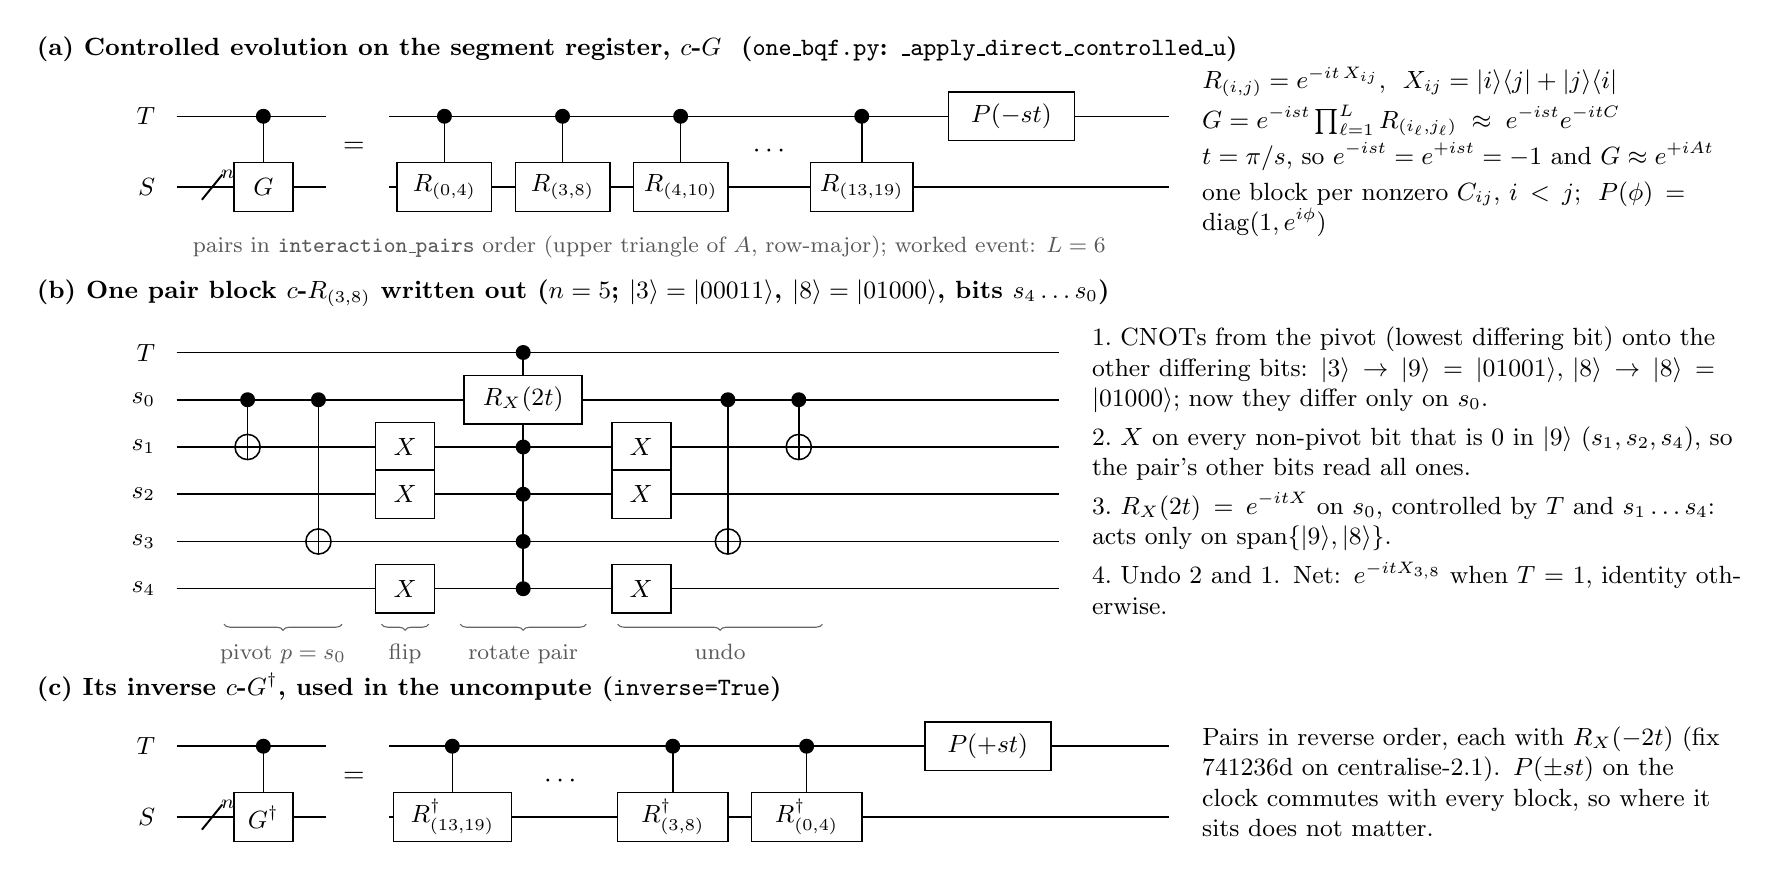
\begin{tikzpicture}[x=1cm,y=1cm]
% (a) the operator as a product of pair blocks
\node[anchor=west,font=\small\bfseries] at (-1.9,1.25) {(a) Controlled evolution on the segment register, $c\text{-}G$ \ (\texttt{one\_bqf.py}: \texttt{\_apply\_direct\_controlled\_u})};
\lab{-0.15}{0.4}{$T$} \lab{-0.15}{-0.5}{$S$}
\wires{0}{1.9}{0.4,-0.5} \slashwire{0.45}{-0.5}{$n$}
\ct{1.1}{0.4} \vl{1.1}{0.4}{-0.5} \gt{1.1}{-0.5}{$G$}
\node at (2.25,0) {$=$};
\wires{2.7}{12.6}{0.4,-0.5}
\ct{3.4}{0.4} \vl{3.4}{0.4}{-0.5} \wg{3.4}{-0.5}{12mm}{$R_{(0,4)}$}
\ct{4.9}{0.4} \vl{4.9}{0.4}{-0.5} \wg{4.9}{-0.5}{12mm}{$R_{(3,8)}$}
\ct{6.4}{0.4} \vl{6.4}{0.4}{-0.5} \wg{6.4}{-0.5}{12mm}{$R_{(4,10)}$}
\node at (7.55,-0.05) {$\cdots$};
\ct{8.7}{0.4} \vl{8.7}{0.4}{-0.5} \wg{8.7}{-0.5}{13mm}{$R_{(13,19)}$}
\wg{10.6}{0.4}{16mm}{$P(-st)$}
\node[font=\small,anchor=west,text width=6.6cm] at (12.9,-0.05) {$R_{(i,j)}=e^{-it\,X_{ij}}$, \ $X_{ij}=|i\rangle\langle j|+|j\rangle\langle i|$\\[2pt] $G=e^{-ist}\prod_{\ell=1}^{L}R_{(i_\ell,j_\ell)}\;\approx\;e^{-ist}e^{-itC}$\\[2pt] $t=\pi/s$, so $e^{-ist}=e^{+ist}=-1$ and $G\approx e^{+iAt}$\\[2pt] one block per nonzero $C_{ij}$, $i<j$; \ $P(\phi)=\mathrm{diag}(1,e^{i\phi})$};
\node[blk] at (6.0,-1.0) {pairs in \texttt{interaction\_pairs} order (upper triangle of $A$, row-major); worked event: $L=6$};
% (b) one pair block, worked: (i,j) = (3,8) on n = 5
\begin{scope}[shift={(0,-3.2)}]
\node[anchor=west,font=\small\bfseries] at (-1.9,1.35) {(b) One pair block $c\text{-}R_{(3,8)}$ written out ($n=5$; $|3\rangle=|00011\rangle$, $|8\rangle=|01000\rangle$, bits $s_4\ldots s_0$)};
\lab{-0.15}{0.6}{$T$}
\lab{-0.15}{0}{$s_0$} \lab{-0.15}{-0.6}{$s_1$} \lab{-0.15}{-1.2}{$s_2$} \lab{-0.15}{-1.8}{$s_3$} \lab{-0.15}{-2.4}{$s_4$}
\wires{0}{11.2}{0.6,0,-0.6,-1.2,-1.8,-2.4}
% CNOT ladder from pivot s0 onto s1, s3
\ct{0.9}{0} \vl{0.9}{0}{-0.6} \tg{0.9}{-0.6}
\ct{1.8}{0} \vl{1.8}{0}{-1.8} \tg{1.8}{-1.8}
% X flips on s1 s2 s4
\gt{2.9}{-0.6}{$X$} \gt{2.9}{-1.2}{$X$} \gt{2.9}{-2.4}{$X$}
% MC-RX
\ct{4.4}{0.6} \ct{4.4}{-0.6} \ct{4.4}{-1.2} \ct{4.4}{-1.8} \ct{4.4}{-2.4} \vl{4.4}{0.6}{-2.4}
\wg{4.4}{0}{15mm}{$R_X(2t)$}
\gt{5.9}{-0.6}{$X$} \gt{5.9}{-1.2}{$X$} \gt{5.9}{-2.4}{$X$}
\ct{7.0}{0} \vl{7.0}{0}{-1.8} \tg{7.0}{-1.8}
\ct{7.9}{0} \vl{7.9}{0}{-0.6} \tg{7.9}{-0.6}
\draw[brace] (0.6,-2.85) -- (2.1,-2.85); \node[blk] at (1.35,-2.98) {pivot $p=s_0$};
\draw[brace] (2.6,-2.85) -- (3.2,-2.85); \node[blk] at (2.9,-2.98) {flip};
\draw[brace] (3.6,-2.85) -- (5.2,-2.85); \node[blk] at (4.4,-2.98) {rotate pair};
\draw[brace] (5.6,-2.85) -- (8.2,-2.85); \node[blk] at (6.9,-2.98) {undo};
\node[font=\small,anchor=west,text width=8.4cm] at (11.5,-0.9) {1.\ CNOTs from the pivot (lowest differing bit) onto the other differing bits: $|3\rangle\to|9\rangle=|01001\rangle$, $|8\rangle\to|8\rangle=|01000\rangle$; now they differ only on $s_0$.\\[3pt]
2.\ $X$ on every non-pivot bit that is $0$ in $|9\rangle$ ($s_1,s_2,s_4$), so the pair's other bits read all ones.\\[3pt]
3.\ $R_X(2t)=e^{-itX}$ on $s_0$, controlled by $T$ and $s_1\ldots s_4$: acts only on $\mathrm{span}\{|9\rangle,|8\rangle\}$.\\[3pt]
4.\ Undo 2 and 1. Net: $e^{-itX_{3,8}}$ when $T=1$, identity otherwise.};
\end{scope}
% (c) inverse
\begin{scope}[shift={(0,-8.0)}]
\node[anchor=west,font=\small\bfseries] at (-1.9,1.15) {(c) Its inverse $c\text{-}G^{\dagger}$, used in the uncompute (\texttt{inverse=True})};
\lab{-0.15}{0.4}{$T$} \lab{-0.15}{-0.5}{$S$}
\wires{0}{1.9}{0.4,-0.5} \slashwire{0.45}{-0.5}{$n$}
\ct{1.1}{0.4} \vl{1.1}{0.4}{-0.5} \gt{1.1}{-0.5}{$G^\dagger$}
\node at (2.25,0) {$=$};
\wires{2.7}{12.6}{0.4,-0.5}
\ct{3.5}{0.4} \vl{3.5}{0.4}{-0.5} \wg{3.5}{-0.5}{15mm}{$R^\dagger_{(13,19)}$}
\node at (4.9,-0.05) {$\cdots$};
\ct{6.3}{0.4} \vl{6.3}{0.4}{-0.5} \wg{6.3}{-0.5}{14mm}{$R^\dagger_{(3,8)}$}
\ct{8.0}{0.4} \vl{8.0}{0.4}{-0.5} \wg{8.0}{-0.5}{14mm}{$R^\dagger_{(0,4)}$}
\wg{10.3}{0.4}{16mm}{$P(+st)$}
\node[font=\small,anchor=west,text width=6.6cm] at (12.9,-0.05) {Pairs in reverse order, each with $R_X(-2t)$ (fix 741236d on centralise-2.1). $P(\pm st)$ on the clock commutes with every block, so where it sits does not matter.};
\end{scope}
\end{tikzpicture}
\end{document}
